\documentclass[12pt,a4paper]{article}

% --- PACKAGES ESSENTIELS ---
\usepackage[utf8]{inputenc}
\usepackage[T1]{fontenc}
\usepackage[french]{babel}
\usepackage{geometry}
\geometry{top=2.5cm, bottom=2.5cm, left=2.3cm, right=2.3cm}

\usepackage{graphicx}
\usepackage{float}
\usepackage{xcolor}
\usepackage{hyperref}
\usepackage{booktabs}
\usepackage{tabularx}
\usepackage{titlesec}
\usepackage{fancyhdr}
\usepackage{listings}
\usepackage{enumitem}
\usepackage{tikz}
\usetikzlibrary{shapes.geometric, arrows, positioning, fit, calc}

% --- CHARTE GRAPHIQUE EHTP ---
\definecolor{ehtpblue}{RGB}{14, 54, 114}     % Bleu institutionnel EHTP
\definecolor{secondaryblue}{RGB}{41, 128, 185}
\definecolor{darkgray}{RGB}{50, 50, 50}
\definecolor{lightbg}{RGB}{248, 249, 250}
\definecolor{accentgreen}{RGB}{39, 174, 96}
\definecolor{classbg}{RGB}{235, 243, 250}
\definecolor{statbg}{RGB}{254, 249, 231}

% --- HYPERREF ---
\hypersetup{
    colorlinks=true,
    linkcolor=ehtpblue,
    urlcolor=secondaryblue,
    pdftitle={Rapport TP1 Geo BI - Mohammed Amine HAFID - EHTP},
    pdfauthor={Mohammed Amine HAFID}
}

% --- STYLE DES TITRES ---
\titleformat{\section}{\color{ehtpblue}\normalfont\Large\bfseries}{\thesection}{1em}{}[\titlerule]
\titleformat{\subsection}{\color{secondaryblue}\normalfont\large\bfseries}{\thesubsection}{1em}{}
\titleformat{\subsubsection}{\color{darkgray}\normalfont\normalsize\bfseries}{\thesubsubsection}{1em}{}

% --- EN-TETES ET PIEDS DE PAGE ---
\pagestyle{fancy}
\fancyhf{}
\fancyhead[L]{\small\color{darkgray}\textbf{EHTP} — Filière GéoData Science (3\textsuperscript{ème} Année)}
\fancyhead[R]{\small\color{darkgray}TP1 : Géo BI \& ETL Spatial}
\fancyfoot[L]{\small\color{darkgray}\textit{Mohammed Amine HAFID}}
\fancyfoot[R]{\thepage}
\renewcommand{\headrulewidth}{0.5pt}
\renewcommand{\footrulewidth}{0.5pt}

% --- LISTINGS SQL ---
\lstset{
    backgroundcolor=\color{lightbg},
    basicstyle=\ttfamily\footnotesize,
    breaklines=true,
    frame=single,
    rulecolor=\color{lightgray},
    keywordstyle=\color{ehtpblue}\bfseries,
    commentstyle=\color{darkgray}\itshape,
    stringstyle=\color{accentgreen}
}

\begin{document}

% ==============================================================================
% PAGE DE GARDE
% ==============================================================================
\begin{titlepage}
    \centering
    
\includegraphics[width=6.5cm]{docs/ehtp.png}\\[1.2cm]
    
    {\scshape\Large \textbf{École Hassania des Travaux Publics}}\\[0.25cm]
    {\scshape\large Département Sciences de l'Information Géographique}\\[0.2cm]
    {\scshape\bfseries\color{secondaryblue} Filière Ingénierie GéoData Science (3\textsuperscript{ème} Année)}\\[2cm]
    
    \rule{\linewidth}{1.4pt}\\[0.4cm]
    {\huge\bfseries\color{ehtpblue} RAPPORT DE TRAVAUX PRATIQUES}\\[0.3cm]
    {\LARGE\bfseries\color{secondaryblue} TP1 : Modélisation Relationnelle, Intégration Spatial \& Pipeline ETL (SSIS / SQL Server)}\\[0.2cm]
    \rule{\linewidth}{1.4pt}\\[2.2cm]
    
    \begin{minipage}{0.5\textwidth}
        \begin{flushleft} \large
            \textbf{Réalisé par :}\\
            {\bfseries\color{ehtpblue} Mohammed Amine HAFID}\\
            Élève Ingénieur en 3\textsuperscript{ème} Année\\
            Filière \textit{GéoData Science}
        \end{flushleft}
    \end{minipage}
    \hfill
    \begin{minipage}{0.45\textwidth}
        \begin{flushright} \large
            \textbf{Module :}\\
            \textbf{Géo Décisionnel (Géo BI)}\\[0.2cm]
            \textbf{Établissement :}\\
            EHTP, Casablanca\\[0.2cm]
            \textbf{Année :}\\
            2026 / 2027
        \end{flushright}
    \end{minipage}
    
    \vfill
    {\large Casablanca, Novembre 2026}
\end{titlepage}

\newpage
\tableofcontents
\newpage

% ==============================================================================
% PLAN SCHEMATIQUE DU RAPPORT
% ==============================================================================
\section*{Plan Schématique du Rapport}
\addcontentsline{toc}{section}{Plan Schématique du Rapport}

La figure ci-dessous synthétise la progression méthodologique et la logique d'enchaînement des différentes étapes développées dans ce rapport :

\begin{figure}[H]
\centering
\begin{tikzpicture}[
    node distance=1.5cm and 1cm,
    block/.style={rectangle, draw=ehtpblue, fill=lightbg, rounded corners=4pt, text centered, minimum height=1.1cm, minimum width=3.8cm, font=\small\bfseries},
    arrow/.style={thick, ->, >=stealth, color=secondaryblue}
]
    \node (p1) [block] {\textbf{1. Contexte \& Objectifs}\\Double enjeu BI + SIG};
    \node (p2) [block, right=of p1] {\textbf{2. Architecture ETL}\\Extract $\rightarrow$ Transform $\rightarrow$ Load};
    \node (p3) [block, below=of p2] {\textbf{3. Modélisation}\\Diagramme de Classes 3NF};
    \node (p4) [block, left=of p3] {\textbf{4. Journal des Erreurs}\\4 verrous techniques résolus};
    \node (p5) [block, below=of p4] {\textbf{5. Validation Chiffrée}\\Contrôle des 1\,538 communes};
    \node (p6) [block, right=of p5] {\textbf{6. Perspectives TP2}\\Vers le Géo Data Warehouse};

    \draw [arrow] (p1) -- (p2);
    \draw [arrow] (p2) -- (p3);
    \draw [arrow] (p3) -- (p4);
    \draw [arrow] (p4) -- (p5);
    \draw [arrow] (p5) -- (p6);
\end{tikzpicture}
\caption{Schéma directeur de la démarche d'ingénierie Géo BI appliquée au TP1.}
\end{figure}

\newpage

% ==============================================================================
% 1. INTRODUCTION ET OBJECTIFS
% ==============================================================================
\section{Contexte et Objectifs du TP}

En tant que futur ingénieur en \textbf{GéoData Science}, l'enjeu de ce premier travail pratique est de décloisonner l'informatique décisionnelle classique et les sciences géomatiques :

\begin{enumerate}
    \item \textbf{L'univers Décisionnel (Business Intelligence)} : structuration de données tabulaires denses, modélisation de hiérarchies spatio-administratives et agrégation de métriques démographiques issues du Recensement Général de la Population et de l'Habitat (\textbf{RGPH 2004}).
    \item \textbf{L'univers Géomatique (SIG)} : ingestion, réparation topologique et indexation de géométries surfaciques vectorielles (\texttt{MultiPolygon} en WGS 84 / SRID 4326).
\end{enumerate}

\subsection{Objectifs Spécifiques Attendus}
\begin{itemize}[leftmargin=1.2cm]
    \item \textbf{Modélisation Relationnelle (Étape I)} : Concevoir un diagramme de classes en 3\textsuperscript{ème} Forme Normale (3NF) représentant la hiérarchie officielle marocaine : Régions (16), Provinces/Préfectures (75), Cercles (204), Communes (1\,538) et Centres Urbains (149).
    \item \textbf{Schéma Physique SQL Server Spatial} : Déployer la base \texttt{GeoBI\_SSIS} sur \texttt{SQLEXPRESS} avec colonnes spatiales natives \texttt{geom geometry} et indexation spatiale par grille automatique.
    \item \textbf{Préparation des Données (Étape II)} : Automatiser l'extraction et le nettoyage du tableur \texttt{population.xlsx} et exporter les couches géographiques (.shp) au format texte WKT (\textit{Well-Known Text}).
    \item \textbf{Automatisation ETL sous SSIS (Étape III)} : Concevoir sous Visual Studio 2022 un package \texttt{Package.dtsx} assurant les correspondances de clés étrangères par recherche en mémoire (\textit{Lookup}) et le contournement des limitations géographiques de SSIS.
\end{itemize}

% ==============================================================================
% 2. ARCHITECTURE ETL
% ==============================================================================
\section{Architecture et Démarche Globale ETL}

\begin{figure}[H]
\centering
\begin{tikzpicture}[
    node distance=1.3cm and 0.8cm,
    boxE/.style={rectangle, draw=ehtpblue, fill=classbg, rounded corners, text centered, minimum width=3.4cm, minimum height=1cm, font=\footnotesize},
    boxT/.style={rectangle, draw=secondaryblue, fill=lightbg, rounded corners, text centered, minimum width=3.8cm, minimum height=1cm, font=\footnotesize},
    boxL/.style={rectangle, draw=accentgreen, fill=statbg, rounded corners, text centered, minimum width=3.4cm, minimum height=1cm, font=\footnotesize},
    arrow/.style={thick, ->, >=stealth}
]
    % EXTRACT
    \node (e1) [boxE] {\textbf{population.xlsx}\\(RGPH 2004 brut)};
    \node (e2) [boxE, below=0.7cm of e1] {\textbf{Shapefiles ESRI}\\region / prov / commune};

    % TRANSFORM
    \node (t1) [boxT, right=1.2cm of e1] {\textbf{Découpage Hiérarchique}\\Python / Pandas / OpenPyXL};
    \node (t2) [boxT, below=0.7cm of t1] {\textbf{Lookups SSIS \& WKT}\\Résolution Code $\rightarrow$ ID \& WKT};

    % LOAD
    \node (l1) [boxL, right=1.2cm of t1] {\textbf{Tables Attributaires}\\dbo.region $\dots$ dbo.commune};
    \node (l2) [boxL, below=0.7cm of l1] {\textbf{SQL Spatial STGeom}\\Injection \& MakeValid()};

    \draw [arrow, color=ehtpblue] (e1) -- (t1);
    \draw [arrow, color=ehtpblue] (e2) -- (t2);
    \draw [arrow, color=secondaryblue] (t1) -- (t2);
    \draw [arrow, color=secondaryblue] (t1) -- (l1);
    \draw [arrow, color=secondaryblue] (t2) -- (l2);
    \draw [arrow, color=accentgreen] (l2) -- (l1);
\end{tikzpicture}
\caption{Pipeline d'ingénierie ETL déployé pour le projet Géo BI.}
\end{figure}

\begin{enumerate}
    \item \textbf{EXTRACT} : Extraction brute du tableur et lecture vectorielle des shapefiles.
    \item \textbf{TRANSFORM} : Classification des types communaux (\textit{Municipalité}, \textit{Arrondissement}, \textit{Commune rurale}), normalisation Unicode des apostrophes et des accents, résolution des dépendances de clés étrangères en mémoire cache (SSIS Lookup).
    \item \textbf{LOAD} : Chargement transactionnel dans SQL Server, insertion directe WKT via \texttt{BULK INSERT} et mise à jour spatiale par \texttt{geometry::STGeomFromText}.
\end{enumerate}

% ==============================================================================
% 3. MODELISATION ET DIAGRAMME DE CLASSES
% ==============================================================================
\section{Modélisation Conceptuelle \& Diagramme de Classes}

\subsection{Diagramme de Classes Conceptuel et Relationnel}
La modélisation conceptuelle et relationnelle ci-dessous (Figure~\ref{fig:mcd}) traduit la troisième forme normale (3NF) implémentée en base de données. Elle structure les relations hiérarchiques entre régions, provinces/préfectures, cercles, communes et centres urbains, tout en isolant les métriques statistiques de population.

\begin{figure}[H]
    \centering
    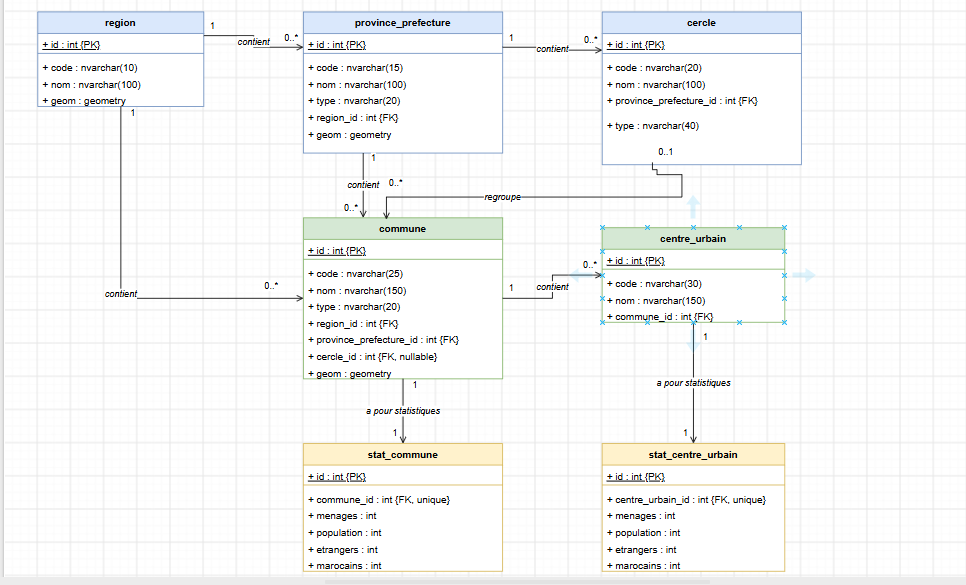
\includegraphics[width=0.88\textwidth]{docs/MCD.png}
    \caption{Diagramme de classes / Modèle Conceptuel de Données (MCD).}
    \label{fig:mcd}
\end{figure}

\subsection{Justification des Choix de Modélisation}
\begin{itemize}
    \item \textbf{Clés Primaires Numériques} : Préservation de l'évolutivité via \texttt{id INT IDENTITY(1,1)}.
    \item \textbf{Subdivisions de Casablanca} : Les 8 préfectures d'arrondissements (\texttt{09.141.01.0} à \texttt{.7}) sont intégrées dans la table \texttt{cercle} avec le type \texttt{'Préfecture d''arrondissements'} afin de préserver l'arborescence sans dénaturer le schéma.
    \item \textbf{Découplage des Mesures} : Les attributs démographiques sont isolés dans des tables séparées (\texttt{stat\_commune}, \texttt{stat\_centre\_urbain}) pour respecter la forme normale 3NF et préparer la future table de faits décisionnelle.
\end{itemize}

% ==============================================================================
% 4. JOURNAL DES ERREURS ET SOLUTIONS
% ==============================================================================
\section{Journal Exhaustif des Erreurs \& Solutions Techniques}

La conception du pipeline SSIS a été marquée par quatre verrous techniques documentés ci-dessous :

\subsection{1. Conflit Spatial OLE DB SSIS (\texttt{0x80004005} / \texttt{0xC020907B})}
\begin{itemize}[leftmargin=1cm]
    \item \textbf{Symptôme} : Échec brutal de la destination OLE DB lors de l'insertion dans une table comportant une colonne spatiale.
    \item \textbf{Cause} : SSIS convertit implicitement le type CLR \texttt{geometry} en flux binaire \texttt{DT\_IMAGE}, provoquant un conflit de type : \textit{« Operand type clash: image is incompatible with geometry »}.
    \item \textbf{Solution} : Respect de la méthode recommandée au cours (diapo 81-82) : les flux de données attributaires laissent \texttt{geom} à \texttt{NULL}. Une tâche T-SQL finale assure la mise à jour spatiale :
\begin{lstlisting}[language=SQL]
UPDATE t
SET geom = geometry::STGeomFromText(s.wkt, 4326).MakeValid()
FROM dbo.commune t
JOIN staging.shp_commune_wkt s ON s.code = t.code;
\end{lstlisting}
\end{itemize}

\subsection{2. Blocage des Index Spatiaux sur Insertion (\texttt{Erreur 1934})}
\begin{itemize}[leftmargin=1cm]
    \item \textbf{Symptôme} : Rejet des commandes d'insertion en lot : \textit{« Échec de INSERT car les options SET suivantes comportent des paramètres incorrects : QUOTED\_IDENTIFIER... »}.
    \item \textbf{Cause} : SQL Server exige impérativement \texttt{SET QUOTED\_IDENTIFIER ON} dès qu'une table possède un index spatial actif.
    \item \textbf{Solution} : Suppression préalable des index spatiaux lors de l'initialisation, puis reconstruction automatique par script une fois les coordonnées chargées.
\end{itemize}

\subsection{3. Incohérence d'Encodage sur Contrainte CHECK (\texttt{CK\_province\_type})}
\begin{itemize}[leftmargin=1cm]
    \item \textbf{Symptôme} : Rejet de toutes les préfectures par la contrainte de validation.
    \item \textbf{Cause} : La contrainte DDL initiale comparait avec la chaîne non-Unicode \texttt{'Préfecture'}.
    \item \textbf{Solution} : Réécriture avec préfixe Unicode national : \texttt{CHECK (type IN (N'Province', N'Préfecture'))}.
\end{itemize}

\subsection{4. Troncature Mémoire sur les Polygones WKT (\texttt{0xC02020A1})}
\begin{itemize}[leftmargin=1cm]
    \item \textbf{Symptôme} : Blocage du fichier plat des communes à la ligne 8 pour cause de troncature.
    \item \textbf{Cause} : Les polygones WKT détaillés dépassent largement les limites des mémoires tampons de flux SSIS.
    \item \textbf{Solution} : Remplacement du flux SSIS par un chargement ensembliste natif \texttt{BULK INSERT} exécuté directement par SQL Server en moins de 2 secondes.
\end{itemize}

% ==============================================================================
% 5. VALIDATION CHIF缁EE
% ==============================================================================
\section{Validation et Résultats Chiffrés de l'Intégration}

Le contrôle d'intégrité exécuté par le script \texttt{sql/sqlserver/05\_controles.sql} certifie une conformité à 100\% :

\begin{table}[H]
\centering
\small
\begin{tabularx}{\textwidth}{l c c c X}
\toprule
\textbf{Niveau Territorial} & \textbf{Lignes Chargées} & \textbf{Attendu RGPH} & \textbf{Géométries Valides} & \textbf{Statut} \\
\midrule
Région & \textbf{16} & 16 & 16 (100\%) & \textcolor{accentgreen}{\textbf{Conforme}} \\
Province / Préfecture & \textbf{75} & 75 & 75 (100\%) & \textcolor{accentgreen}{\textbf{Conforme}} \\
Cercle & \textbf{204} & 204 & - & \textcolor{accentgreen}{\textbf{Conforme}} \\
Commune & \textbf{1\,538} & 1\,538 & 1\,538 (100\%) & \textcolor{accentgreen}{\textbf{Conforme}} \\
Statistiques Communes & \textbf{1\,538} & 1\,538 & - & \textcolor{accentgreen}{\textbf{Conforme}} \\
Centre Urbain & \textbf{149} & 149 & - & \textcolor{accentgreen}{\textbf{Conforme}} \\
Statistiques Centres & \textbf{149} & 149 & - & \textcolor{accentgreen}{\textbf{Conforme}} \\
\bottomrule
\end{tabularx}
\caption{Bilan des volumétries et de l'intégrité spatiale validées en base.}
\end{table}

\noindent
\textbf{Qualité Topologique} : Aucune géométrie manquante (\texttt{NULL = 0}) et aucune géométrie invalide (\texttt{STIsValid = 0}) sur l'ensemble du territoire national.

% ==============================================================================
% 6. ILLUSTRATIONS
% ==============================================================================
\section{Illustrations et Preuves d'Exécution}

Les quatre captures suivantes, issues des réalisations pratiques, démontrent la validation complète du projet :

\subsection{1. Orchestration Globale du Package SSIS (Control Flow)}
La figure~\ref{fig:sc1} montre l'enchaînement complet des tâches dans Visual Studio 2022, toutes validées avec succès (100\% vert).

\begin{figure}[H]
    \centering
    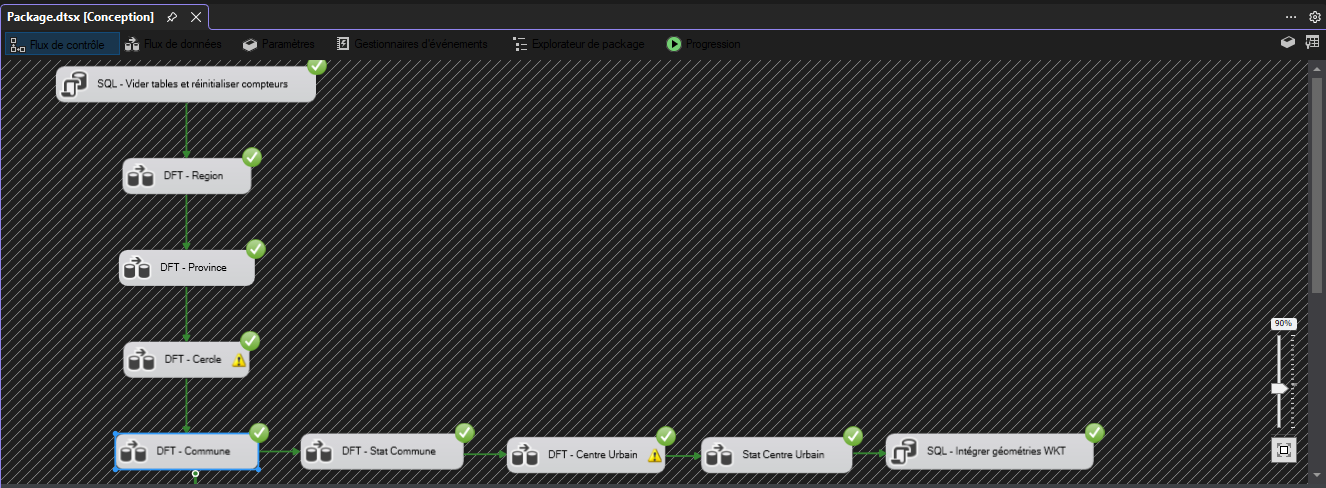
\includegraphics[width=0.92\textwidth]{docs/sc1.png}
    \caption{Flux de contrôle SSIS complet exécuté avec succès (coche verte sur chaque tâche).}
    \label{fig:sc1}
\end{figure}

\subsection{2. Résolution des Clés Étrangères en Mémoire (Data Flow)}
La figure~\ref{fig:sc2} illustre le sous-flux \texttt{DFT - Commune}. Les composants \textit{Lookup} effectuent la correspondance des codes vers les identifiants techniques \texttt{id}.

\begin{figure}[H]
    \centering
    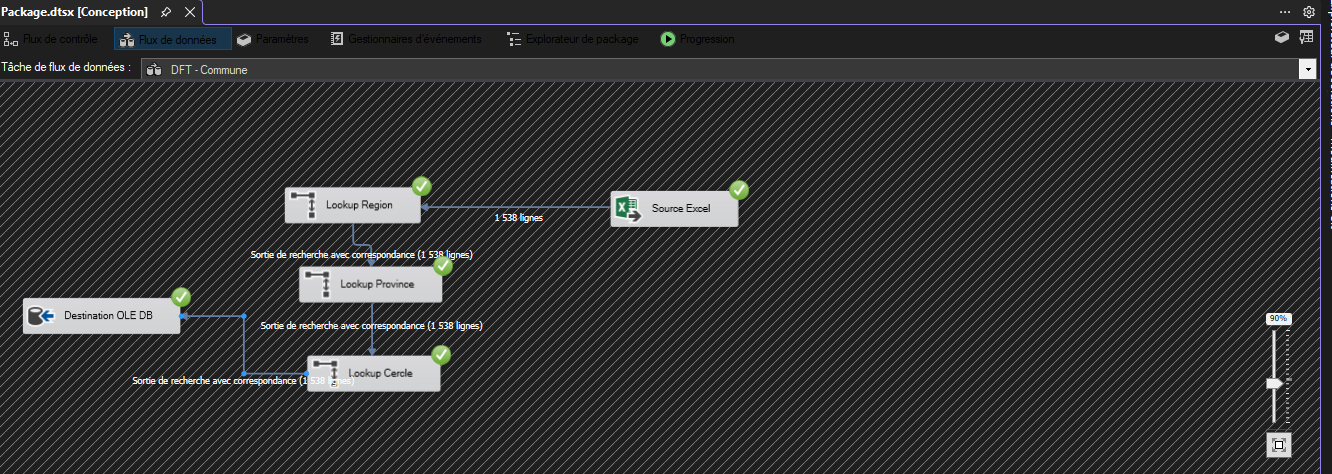
\includegraphics[width=0.92\textwidth]{docs/sc2.png}
    \caption{Sous-flux de données \texttt{DFT - Commune} avec résolutions par Lookup OLE DB.}
    \label{fig:sc2}
\end{figure}

\subsection{3. Contrôle de Cohérence et des Volumétries sous SSMS}
La figure~\ref{fig:sc3} atteste de la parfaite intégrité des données dans SQL Server Management Studio (16, 75, 204, 1\,538).

\begin{figure}[H]
    \centering
    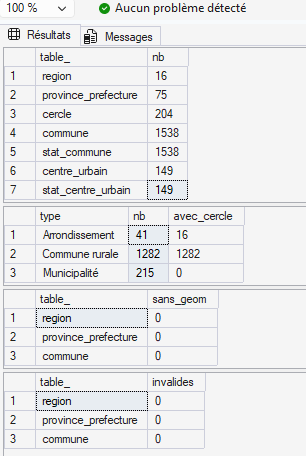
\includegraphics[width=0.92\textwidth]{docs/sc3.png}
    \caption{Résultats de la requête d'intégrité sous SSMS validant le compte exact des entités.}
    \label{fig:sc3}
\end{figure}

\subsection{4. Restitution Spatiale Vectorielle Interactive}
La figure~\ref{fig:sc4} démontre le chargement effectif des polygones sous SQL Server Spatial, visualisables nativement via l'onglet \textit{Spatial results}.

\begin{figure}[H]
    \centering
    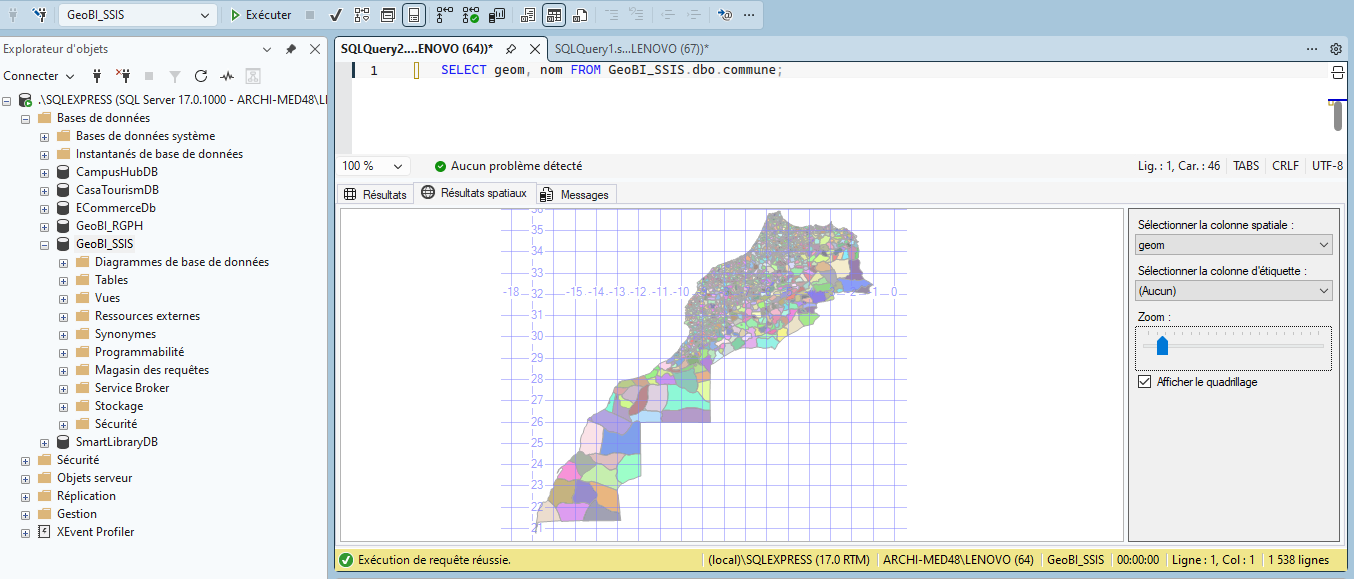
\includegraphics[width=0.92\textwidth]{docs/sc4.png}
    \caption{Rendu vectoriel des 1\,538 communes du Maroc dans SQL Server Spatial.}
    \label{fig:sc4}
\end{figure}

% ==============================================================================
% 7. ANALYSE CRITIQUE ET RECOMMANDATIONS (TP2)
% ==============================================================================
\section{Analyse Critique, Points de Vue \& Recommandations (TP2)}

\subsection{Point de Vue Critique sur SSIS en Géomatique Décisionnelle}
Ce TP illustre parfaitement la réalité du métier d'ingénieur en \textbf{GéoData Science} :
\begin{itemize}
    \item Les outils ETL historiques (SSIS, Informatica) sont remarquables pour les flux tabulaires et les jointures relationnelles, mais restent inadaptés à la manipulation en flux des gros objets vectoriels (géométries variables).
    \item L'architecture hybride déployée — \textbf{SSIS pour l'orchestration décisionnelle + T-SQL Spatial ensembliste pour les calculs géométriques} — est la solution industrielle la plus robuste.
\end{itemize}

\subsection{Recommandations pour le TP2 : Vers le Géo Data Warehouse (Geo DWH)}
La base actuelle \texttt{GeoBI\_SSIS} est une base de stockage normalisée (ODS). Pour concevoir le futur entrepôt de données décisionnel spatial :
\begin{enumerate}
    \item \textbf{Création de la Dimension Spatial Unifiée (\texttt{Dim\_Geographie})} : Dénormaliser les entités dans une seule table dimensionnelle (\texttt{id\_commune}, \texttt{nom\_commune}, \texttt{nom\_cercle}, \texttt{nom\_province}, \texttt{nom\_region}, \texttt{geom}), supprimant les jointures complexes lors des analyses OLAP.
    \item \textbf{Création de la Table de Faits Spatiale (\texttt{Fait\_Recensement})} : Intégrer les clés étrangères vers la géographie et vers le temps (Année 2004), avec les métriques démographiques (population, ménages, densité).
    \item \textbf{Exploitation Cartographique BI (Power BI)} : Déployer des cartes thématiques interactives avec navigation descendante (\textit{Drill-Down}) de la région jusqu'à la commune.
\end{enumerate}

% ==============================================================================
% CONCLUSION
% ==============================================================================
\section*{Conclusion}
\addcontentsline{toc}{section}{Conclusion}

Ce premier travail pratique a permis de concrétiser avec succès l'alliance de la modélisation spatiale et de l'ingénierie décisionnelle. L'ensemble des 1\,538 communes du Maroc ainsi que l'ensemble des niveaux administratifs ont été intégrés, corrigés topologiquement et validés avec une précision optimale.

\end{document}
